\chapter{Power Plant Cost Model Preparation}\label{ch4:cm_prep}

\section{EGS Expansion Concept}\label{ch4:cm_concept}
\subsection{Lightning Dock EGS}

Lightning Dock (Section \ref{ch2:lightning_dock}) is presently the only commercial power plant operating in the state of New Mexico. The net generating capacity after its first phase of development was 4 MW in 2013, with the expectation of upgrading to 10 MW in a second development phase that never came to fruition. Instead, the facility underwent a significant refit in 2018, resulting in a net capacity of 11.2 MW generated entirely from hydrothermal brine production \citep{bonafin_repowering_2019}. 

Department of Energy-funded efforts to characterize the geothermal resources in the Animas Valley, NM revealed the presence of two different thermal reservoirs: the hydrothermal resource targeted by Lightning Dock where deep geothermal fluids ascend along the Animas Valley Fault complex to $\approx$365-1000 m depth, and a secondary interval at $\approx$900-1200 m depth that requires permeability enhancement for production \citep{schochet_development_2001}. The Horquilla limestone formation defines the second reservoir, estimated to span a minimum volume of 6 cubic km based on conservative figures. By one proprietary study completed in 2001 for Ormat Technologies, a commercial geothermal company, the Horquilla has a 88\% probability of 6 MW in recoverable electricity generation potential \citep{schochet_development_2001}.

\citet{schochet_development_2001} proposed the construction of a 6 MW hybrid power plant combining hydrothermal and EGS-sourced power generation a decade before operations commenced at Lightning Dock. In their development plan, they noted several benefits of pursuing EGS in this location:
\begin{itemize}[itemsep=2pt]\label{ch4:ld_egs_support}
    \item Relatively shallow resource drives lower drilling costs
    \item EGS water requirements are attainable from paired hydrothermal operations
    \item A comprehensive initial assessment determined no significant environmental degradation is expected from geothermal operations
    \item Lightning Dock has direct access to in-place transmission lines  
    \item Opportunities exist for electricity sales to local users
    \item Purchase agreements with regional utilities are incentivized by NM legislation
\end{itemize}

As suggested by this list, the conditions at Lightning Dock offer a nearly ideal test case for an EGS proof of concept on a manageable scale. Historical land utilization in the area is primarily agricultural with few residences, so risk is low for any adverse impact on an existing population. In addition, use of a binary cycle design as proposed by \citet{schochet_development_2001} offers the potential for power production with zero GHG emissions.  

In this thesis, the \citeauthor{schochet_development_2001} concept is revisited with the existing geothermal production at Lightning Dock kept in mind; rather than building a new hybrid facility, the revised concept involves targeting the deeper reservoir as a near-hydrothermal field EGS (NF-EGS) development with a tie-back to the current Lightning Dock facility. Stepping out from the hydrothermal zone in proximity to the Animas Valley Fault complex, thermal conditions settle to a high background geothermal gradient between $\approx$ 80-120 K/km based on boreholes TG 56-14 and TG 12-7 \citep{cunniff_final_2003} -- certainly high enough to support geothermal capture. These conditions make for an interesting case study on risk mitigation options for EGS production planning.

Public records regarding power generation at Lightning Dock provide some guidance on the appropriate size for an EGS expansion. After phase 1 development, the plant produced 4 MW. An additional 6 MW was slated for phase 2, but re-powering of the plant actually added 7 MW to the capacity after several years of development stasis \citep{think_geoenergy_turboden_2020}. \citeauthor{schochet_development_2001} originally proposed a 6 MW hybrid plant for the site, but they also noted 6 MW from the Horquilla was likely understating the full reservoir potential \citeyear{schochet_development_2001}. In consideration of the step-wise trajectory of plant improvements and assessment of available thermal resource, this case study targets 5 MW as a expansion goal. 

\subsection{New Mexico Electricity Demand}
Pursuing the expansion of a power plant requires sufficient demand to ensure total revenue offsets project expenses. Fortunately, New Mexico regulations support the further development of geothermal power production in the state. Specifically, the Energy Transition Act signed in 2019 updated the New Mexico \acrlong{rps} (\acrshort{rps}) to go zero-carbon by 2050, with milestone targets along the way \citep{lillian_new_2019}. The RPS dates back to the Renewable Energy Act passed in 2004 and comes with several carve-outs, including a 30\% requirement for wind energy, 20\% for solar, and 5\% for other renewables like geothermal \citep{dsire_dsire_2021}. Public Service Company of New Mexico (PNM) is the state’s largest energy provider and services the Lordsburg area where Lightning Dock is located. PNM and Cyrq Energy currently share a 20-year \acrlong{ppa} (\acrshort{ppa}) for electricity generated at Lightning Dock. The PPA has gone through amendments over time to update both the wattage supplied to PNM and the pricing structure per MWh \citep[e.g.,][]{pnm_pnm_2014,stanfield_new_2017}. This indicates a PPA can be revisited if conditions change, which is an important aspect to consider when modeling project financials. 
In addition to the RPS requirement for a diversified renewables portfolio, coal power plants across the state face mandated shut-downs as a consequence off the Energy Transition Act. Coal currently supplies a large fraction ($\approx$ 45\%) of electric power sector consumption in New Mexico (Figure \ref{fig:nm_energy_consumption}). The supply gap introduced as coal-based production ramps down to zero could more than compensate for a 5 MW addition of no-emissions energy to the New Mexico grid.

\begin{figure}[!htp]
\centering
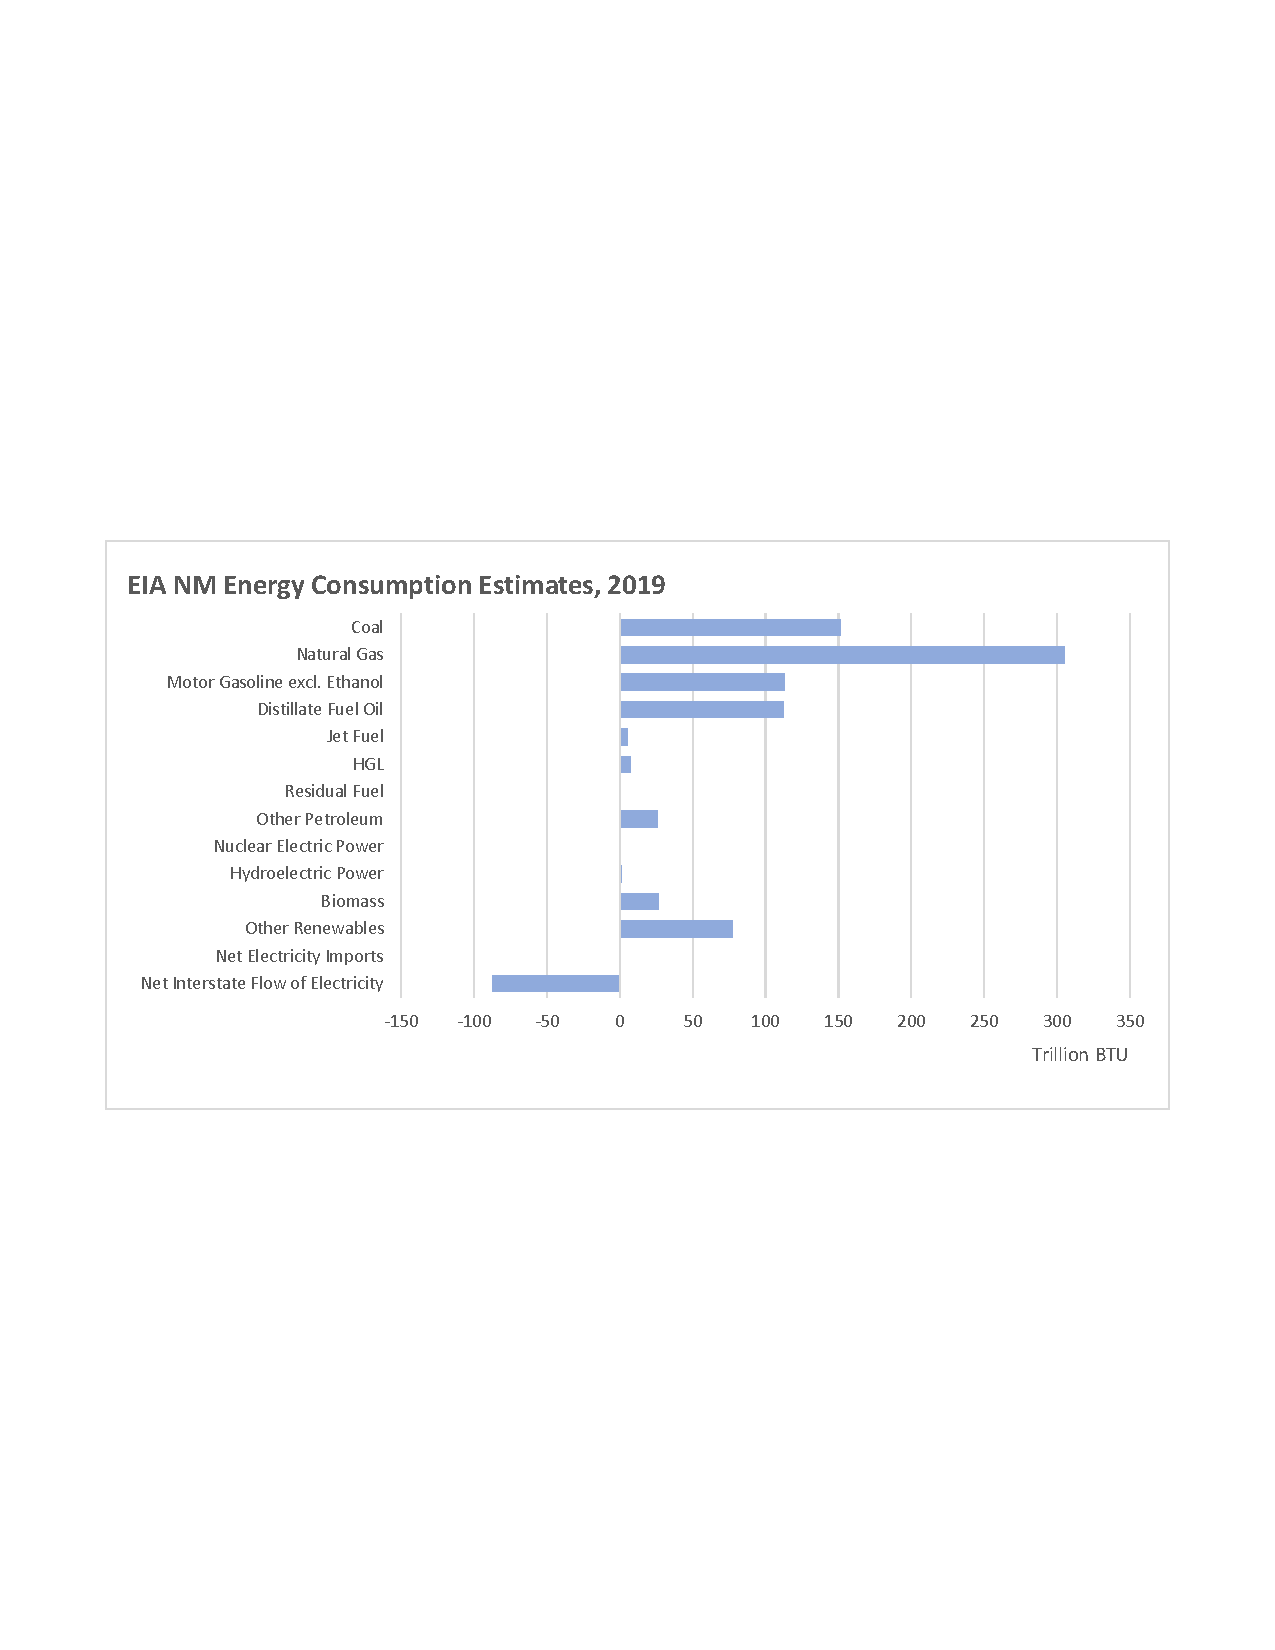
\includegraphics[width=\textwidth]{templates/images/Figure-EIA_NM_Energy_Consumption.pdf}
\caption[NM energy consumption]{Energy consumption by source for New Mexico. Adapted from data and graphics reported by the EIA \protect\citep{eia_new_2021}.}
\label{fig:nm_energy_consumption}
\end{figure}

\subsection{Modular Geothermal}

Limiting this expansion to a single 5 MW facility defines one design alternative, but others exist as well. One flexible option uses modular power plant technology that has recently captured the attention of high-stakes investors across the world (Shieber, 2019). Climeon, for example, has engineered a compact binary cycle unit capable of 150 kW of generated electricity using inlet fluid temperatures rated up to 120℃ and flow rates of up to 35 kg/s \citep{climeon_climeon_2021}. These units can be combined into a larger deployable Power Block for 1050 kW of generated electricity \citep{winther_power_2018} (Figure 4). Power plants can now be treated like multi-unit assemblages, installed all at once or over an extended period of time based on operator needs (Figure 5) (Climeon, 2018)





As discussed in Section XX, cost models can provide insights into the potential value gained or lost by a proposed facility before construction begins.

ailable 
Well-established geothermal cost models like GETEM provide a highly-parameterized but deterministic view of the cost and investment opportunity given a defined geothermal resource and development concept (Entingh et al., 2006). Other models may apply different assumptions or mathematical treatments for various facets of the system, but they uniformly offer a one-track aspect to how the project unfolds over its lifecycle (see Section XX). In the cost model discussed below, the economic analysis includes a stochastic treatment of uncertainties using probability distributions. In addition, it incorporates flexibility rules for decision-making under changing conditions.  


Explicitly sampling from the range of possible values for model-sensitive variables as well as including real option decision rules in a geothermal cost model could provide new insights into project viability and execution strategy missing from these previous approaches.

that utilizes binary cycle modules like the Climeon Power Block, with a single open-loop EGS injector-producer doublet per module. 



Performing flexible design analysis with provides value to engineering projects in a number of ways. First, flexible design recognizes and incorporates uncertainty by replacing single value estimates with realistic distributions for model variables. This enables a model to describe a representative range of possible outcomes when simulated many times over. Flexibility also provides the opportunity to execute real options, where design updates triggered by changing conditions capture upside potential or mitigate against downside risks. Designs need not be static, and real options can offer a means to greatly increase the expected value of a project (de Neufville \& Scholtes, 2011).
 Explicitly sampling from the range of possible values for model-sensitive variables as well as including real option decision rules in a geothermal cost model could provide new insights into project viability and execution strategy missing from these previous approaches.




\section{Flexible Cost Model Structure}\label{ch4:cm_structure}

This thesis considers a simplified model developed in Microsoft Excel to represent the primary sources of cost and revenue for a geothermal power plant expansion. Geothermal cost models typically report Levelized Cost of Electricity (LCOE) for simple comparison with other renewable options, however LCOE is standardized to represent the total lifetime costs incurred by a power plant normalized by the total lifetime power generation from start-up to plant decommissioning. LCOE is not an intuitive metric for communicating projected gains or losses under different designs or future scenarios from the perspective of plant operator. Instead, this analysis uses \acrlong{npv} (\acrshort{npv}), a simple measure of project lifetime worth that accounts for the time value of money through use of a single interest rate for borrowing and deposits, the discount rate \citep[p.\ 195-215]{de_neufville_flexibility_2011}. Here, "present value" refers to a 2020 cost basis. For power generation over a 30-year lifespan \citep{entingh_volume_2006}, this takes the cost model out to 2050, which is a common benchmark year for future projections. 

\subsubsection{Model Formulation}
Following extensive previous work on geothermal cost modeling \citep[e.g.,][]{augustine_hydrothermal_2009, beckers_introducing_2013, tester_economic_1990, tester_future_2006}, this thesis divides cash inflow and outflow for geothermal power generation into the following components:

\begin{equation}
    \label{eq:npv_components}
    \begin{aligned}
    NPV &= Rev - CAPEX_{pp} - CAPEX_{dc} - CAPEX_{exp} \\ 
        &\qquad- CAPEX_{dist} - CAPEX_{stim} - OPEX \\
    \text{where:}\\
    Rev &= capacity\ (kWh) \times PPA\ \left(\frac{\$}{kWh}\right) \\
    CAPEX_{pp} &= power\ plant\ costs\ \left(\frac{\$}{kWe}\right) \times
    avg\ net\ power\ per\ unit\ (kWe)\\
    CAPEX_{dc} &= drilling\ costs\ \left(\frac{\$}{well}\right) \times 2\ (wells\ per\ doublet)\\
    CAPEX_{exp} &= f(drilling\ costs),\ where\ f\ is\ a\ linear\ function\\
    CAPEX_{dist} &= D\ \left(\frac{\$}{well}\right) \times enthalpy\ drop,\ where\ D\ is\ a\ constant\\
    CAPEX_{stim} &= S\ \left(\frac{\$}{well}\right) \times 2\ (wells\ per\ doublet)\\
    OPEX &= Labor\ \left(\frac{\$}{year}\right)+ Plant\ O\&M\ \left(\frac{\$}{year}\right)\\
    &\qquad+ Field\ O\&M \left(\frac{\$}{year}\right) + Water\ O\&M \left(\frac{\$}{year}\right)
    \end{aligned}
\end{equation}

\subsubsection{Model Parameters}

In order to estimate the values of these components, the following parameters were defined for a deterministic cost model. The values selected are reflective of the Animas, NM region, the Lightning Dock facility, and limits on components of the system to the best of the author's knowledge.

